%*************************************************************************************
%
% 2012/08/13
%
% Kei Moriya (Indiana University)
%
% Documentation for gammaKKAmpTools
%
%*************************************************************************************

\documentclass[11pt]{article}
\usepackage{amsmath}
\usepackage{amssymb}
\usepackage{graphicx}
\usepackage{pifont}
\usepackage{color}
\usepackage{amssymb}
\usepackage{subfig}

\textheight 8.0in
\topmargin 0.0in
\textwidth 6.0in
\oddsidemargin 0.25in
\evensidemargin 0.25in

%------------------------     LaTeX commands     ---------------------------------%
% these 3 packages, pifont, graphicx, and color were put in so I can
% use the "comment" command below. Take out if necessary.
\DeclareGraphicsRule{.pdftex}{pdf}{.pdftex}{}
\DeclareGraphicsRule{.pdftex_t}{pdf}{.pdftex}{}
\DeclareGraphicsRule{.gif}{gif}{}{}

\newcommand{\comment}[1]{\textcolor{red}{\ding{110}\ding{43} #1}}
\newcommand{\AmpTools}{{\tt{AmpTools}}}

%*************************************************************************************
%                                                                                    *
%                              Start of main document                                *
%                                                                                    *
%*************************************************************************************
\begin{document}

% To get line numbers using lineo package
% \linenumbers

\title{Example Analysis Using \AmpTools{} for $\gamma KK$}
\author{Kei Moriya\footnote{kmoriya@indiana.edu} \\
  Department of Physics, Indiana University, Bloomington, IN 47403}
\date{\today}

\maketitle

\begin{abstract}
This is documentation for an example of using the \AmpTools{} package
for the analysis of $J/\psi (\psi') \to \gamma KK$. All programs are
documented, and usage is shown.
\end{abstract}

%*************************************************************************************
%                                                                                    *
%                                   Introduction                                     *
%                                                                                    *
%*************************************************************************************
\section{Introduction}

This document illustrates how to quickly start doing analyses with the
use of the \AmpTools{} package. The example we will use is $J/\psi
(\psi') \to \gamma K K$, and we are interested in a mass-independent
analysis. In reality, the above reaction will be restricted to states
of $0^{++}, 2^{++}, 4^{++}, \cdots$ for $KK = K_{S}^{0} K_{S}^{0}$,
but nontheless, for illustration purposes we will show an example of
how the decay will look if we have the $KK$ system going to a spin-$1$
state.

This tutorial should have been downloaded together with the
\AmpTools{} package. Since this tutorial is based on the Dalitz plot
analysis tutorial also included, it is recommended that the Dalitz
plot tutorial be worked out first, to familiarize yourself
with the \AmpTools{} package.

The overall directory structure is set up as follows. The directories
gammaKKAmp, gammaKKDataIO, and gammaKKPlot include all of the
necessary files to create the libraries used by this example. The
top-level Makefile will create all of these libraries. The directory
gammaKKExe contains all of the programs that need to be run in this
example tutorial, and these programs are \textit{not} included in the
top-level Makefile. Go to this directory and type make to create the
executables. The directory run will contain configuration files needed
for generating physics events and fitting. Also included is a file
run.sh that can be used to run all example executables at once.

%*************************************************************************************
%                                                                                    *
%                                  Preliminaries                                     *
%                                                                                    *
%*************************************************************************************
\section{Preliminaries}

To run the tutorial, you will need the packages {\tt ROOT}, {\tt
  CLHEP}, {\tt AmpTools} set up correctly. Make sure the environment
variables {\tt ROOTSYS}, {\tt CLHEP\_INCLUDE\_DIR}, {\tt AMPTOOLS} are
set correctly. The final variable to set is {\tt GAMMAKK}, which can
be set by sourcing the file setup\_gammaKK.csh in the top directory.

Once these are set up, type make in the top directory to create all of
the necessary libraries. Next, move to the gammaKKExe directory and
type make to create all of the executables. Finally, move to the run
directory and run the script run.sh to run all of the executables in
order.

For the file run.sh, if you uncomment the definition of the variable
{\tt VERBOSE} at the top of the file, the script will stop at the end
of each stage, so that you can understand what the output was, rather
than have everything fly by on your screen at once.

%*************************************************************************************
%                                                                                    *
%                                Directory Structure                                 *
%                                                                                    *
%*************************************************************************************
\section{Directory Structure}

As explained in the Introduction, the tutorial is structured so that
the source files for all libraries are contained in gammaKKAmp,
gammaKKDataIO, and gammaKKPlot, while the executables are in
gammaKKExe.

\subsection{Libraries}
Here we will view the files that create the libraries.

\begin{itemize}
\item gammaKKDataIO

This directory contains the files gammaKKDataReader and
gammaDataWriter, which allows the user to read in and write out data
to and from files. The DataReader and DataWriter formats are specified
so that the user has complete freedom in choosing how the data is
formatted.

For gammaKKDataReader, the data is read in in the format of
$4$-vectors for each event from a TTree that contains each
component of all $4$-vectors.

For gammaKKDataWriter, the function \\
{\tt{writeEvent( const Kinematics \& kin)}} \\
will read in each event. The Kinematics object is used throughout the
\AmpTools{} package, and contains a
         {\tt{std::vector<HepLorentzVector>}} for that event. The
         components of the $4$-vectors are written out into a TTree,
         which can in turn be read in by a gammaKKDataReader.

\item gammaKKPlot

This directory contains only gammaKKPlotGenerator, which is used to
plot the results of a fit done in this tutorial. The
gammaKKPlotGenerator class inherits from PlotGenerator in \AmpTools,
and will implement the virtual function {\tt{fillProjections}}. The
executables that will use this class are plotResults and
fitAmplitudesMassBins in gammaKKExe.

\item gammaKKAmp

This directory contains all of the necessary tools needed to generate
physics distributions. Some, like clebschGordan and wignerD are rather
obvious. NBodyPhaseSpaceFactory will generate events based on phase
space, and return a {\tt{std::vector <HepLorentzVector>}} for that
event.

The other files in this directory are for generating specific
amplitudes that involve physics. For this tutorial we will use two
amplitudes, gammaKKHelicityAmp and MultipoleAmps. gammaKKHelicityAmp
will take in as arguments
\begin{itemize}
\item $J$: spin of the $KK$ resonance
\item $\mu$: helicity of the $KK$ resonance ($|\mu| \leq J$)
\item $M$: the $z$-projection of the spin of the initial state
  $J/\psi$ or $\psi'$
\item $\lambda$: the final helicity of the photon ($\lambda = \pm 1$)
\end{itemize}

The helicity amplitudes are very useful in that given a reaction, it
is a simple exercise to write down what that amplitude is. On the
other hand, there is no a priori relation between the strengths of the
different helicity amplitudes (save those related by parity), so it is
difficult to have a physical intuition of the relative strengths.

The class MultipoleAmps will take in as arguments
\begin{itemize}
\item $J$: spin of the $KK$ resonance
\item $J_{\gamma}$: total angular momentum of the photon
\item $M$: the $z$-projection of the spin of the initial state
  $J/\psi$ or $\psi'$
\item $\lambda$: the final helicity of the photon ($\lambda = \pm 1$)
\end{itemize}

Note that due to conservation of angular momentum, $|J - J_{\gamma}|
\leq 1$, where $1$ is the spin of the initial $J/\psi$ or
$\psi'$. Since the helicity of the photon is always $\lambda = \pm 1$
due to its having no mass, $J_{\gamma}$ can never be $0$. These put
restrictions on what values $J_{\gamma}$ can take for a specific
reaction For example, for $J=0$, $J_{\gamma} = 1$ only, for $J=1$,
$J_{\gamma} = 1, 2$, for $J=2$, $J_{\gamma} = 1, 2, 3$, and so on.

The strength of the multipole amplitudes are related to the helicity
amplitudes by a unitary transformation that conserves the overall
strength of the reaction. Although the
multipole basis is rather complicated due to its containing many sums
and coefficients, physics models can give arguments that the lower
multipoles will dominate in certain reactions, and in this case it is
useful to have amplitudes where a hierarchy is expected.

Further details on the relation of helicity and multipole amplitudes
will be given in a later section, as this will give many insights into
how the physics works.

\end{itemize}

\subsection{Executables}
Here we will view the executables that will be used.

\begin{itemize}

  \item generatePhaseSpace

    A class that will generate any number of phase space
    events for a given reaction. This program will make use of
    gammaKKDataWriter to write out the event $4$-vectors into a ROOT
    file using a TTree. The arguments taken in are
    \begin{itemize}
      \item output ROOT file name
      \item number of events
    \end{itemize}

    For the actual generation of phase space events, the class
    NBodyPhaseSpace contained in the directory gammaKKAmp is
    used.
    % // -----------------------------------------------------------
    % //       This applies to TGenPhaseSpace only                //
    % This allows for the creation of phase
    % space distributions of up to $20$ particles.
    %Each event is
    %generated with a specific weight, so that when the events are
    %weighted with that weight, we obtain a flat distribution.
    % // -----------------------------------------------------------

  \item generatePhysics

    A class that is very similar to generatePhaseSpace in that it
    generates events according to a flat phase space distribution, but
    will accept or reject these events according to a set of
    amplitudes specified by the user.

    The program will take in as arguments
    \begin{itemize}
      \item configuration file name
      \item output ROOT file name
      \item number of events to sample from
      \item random seed
    \end{itemize}
    The configuration file is parsed, and the appropriate amplitude
    and intensity is calculated for each event. For this to be
    processed properly, each amplitude that is used must be registered
    within the AmplitudeMananger object. Once this is done, the
    intensity of each event will be calculated, and the maximum
    intensity is saved. Since we want the phase space distribution to
    be filled with each event's weight proportional to its intensity,
    we will throw a random number for each event and keep the event
    only if the intensity is higher than the maximum intenstiy
    multiplied by the random number.

    At the end of the program, the program will report how many events
    have been retained for analysis. The kept events are written into
    a ROOT file.

  \item toyAcceptance

    We would like to simulate having a toy Monte Carlo system that
    has finite acceptance across different regions of phase
    space. This program will just read in the $4$-vectors of each
    event, and write out the event with a probability that is
    proportional to the acceptance at that point. The efficiency can
    be whatever the user chooses. In this tutorial we have an
    acceptance that oscillates with the polar angles of the particle
    in the original frame.

    The program will take in as arguments
    \begin{itemize}
      \item input ROOT file name
      \item output ROOT file name
    \end{itemize}

  \item plotData

    This is a simple program that will take in a ROOT file containing
    a TTree created by gammaKKDataReader, and make some basice
    plots. Currently, there are plots for the invariant masses of the
    combination of particles, a Dalitz plot, and a plot for the
    $\gamma$ polar angle in the rest frame.

  \item fitAmplitudesATI

    The program that will do the heavy work of fitting a given data
    file with the amplitudes that are specified in the configuration
    file that is read in. The program reads in
    \begin{itemize}
      \item configuration file name
    \end{itemize}
    and parses the information to do the fit.

    The configuration file will need the following information. First,
    the definition of a fit name must be given, followed by the
    reaction name. The fit name will be used to create the .fit file
    which contains the fit result. Next, the configuration file must
    specify which files are to be used for the generated phase space
    Monte Carlo distribution, the accepted Monte Carlo events, and the
    data file. The normintfile name will be used to create a
    normalization integral file which contains the correlation of the
    different amplitudes in the fit.

    If the fit successfully converges, the files will be written out,
    and the results examined.

  \item plotResults

    This program will use the fit results to create a ROOT file
    containing the histograms that are specified in
    gammaKKPlotGenerator. The histograms will be for the data, the
    accepted Monte Carlo events, and the generated Monte Carlo events,
    based on the fit result.

  \item fitAmplitudesATIMassBins and fitAmplitudesATISplitMassBins

    These programs are designed to do a mass-independent fit to the
    spectrum of $J/\psi \to \gamma K_{S} K_{S}$, where the data is
    binned in the invariant mass of the $K_{S} K_{S}$ system, and a
    fit is done independently for each mass bin.

    Since it is sometimes useful to be able to seed the next mass
    bin's fit by the previous mass bin's fit result, these two
    programs show examples of how to save the current fit results, and
    put them back into the next fit. In both cases, information
    necessary for binning in $K_{S} K_{S}$ mass is given in the same
    cfg file that will be used in the fit. The keyword ``binning'' is
    used with three arguments,
    \begin{itemize}
      \item the number of mass bin
      \item the minimum value
      \item the maximum value
    \end{itemize}
    and this information is extracted within the programs using the
    class ConfigurationInfo.

    fitAmplitudesATIMassBins is designed to read in all of the ROOT
    files necessary (data, generated Monte Carlo events, accepted
    Monte Carlo events), and for each mass bin, it will loop over the
    entire file to determine how many events fit in that mass bin.
    This is done by passing in three arguments into the
    gammaKKDataReader, where the first argument is the file name, and
    the second and third arguments are the mass ranges of the $K_{S}
    K_{S}$ system.

    As the entire ROOT files are read in and the $K_{S} K_{S}$
    invariant mass is calculated for each event in each mass bin, the
    program is rather slow. An example script of using this program is
    provided in the directory gammaKKExe/massBins1.

    The alternative to this method is to split the necessary ROOT
    files into $K_{S} K_{S}$ mass bins before starting the fits, and
    this is what fitAmplitudesATISplitMassBins does. We first need to
    use the program splitByMass to split each of the ROOT files into
    however many bins are necessary. Then, for the actual fitting,
    only the necessary ROOT files for that mass bin are required to be
    read in.

    This method is the quicker of the two, but the downside is that
    you end up with many more data files in your directory. An example
    script using this program is contained in the directory
    gammaKKExe/massBins2.

\end{itemize}

%*************************************************************************************
%                                                                                    *
%                                Running the Programs                                *
%                                                                                    *
%*************************************************************************************
\section{Running the Programs}

In the run directory, a script run.sh has been created that can be
used to run all of the above executables in the correct order, showing
how they were intended to be used. The variable {\tt{VERBOSE}} can be
uncommented, so that the script will stop at the end of each stage.
Here we view what the program does, and what the results are.

\begin{enumerate}
\setcounter{enumi}{-1}

\item make

  First make all of the executables in gammaKKExe to make sure they
  are up to date.

\item generate phase space events

  Using generatePhaseSpace, we generate $10$M phase space events for
  the reaction $J/\psi \to \gamma K_{S}^{0} K_{S}^{0}$.

\item apply toy acceptance to the Monte Carlo events

  Using toyAcceptance, we apply our acceptance to the generated events
  to obtain our acceptend Monte Carlo event sample.

\item create plots of Dalitz distribution for the Monte Carlo events

We use plotData to create plots of the above distributions. The plots
are saved in the figures directory.

\item generate physics events

We generate $1$M physics events according to the physics that we
specify in our configuration file. We can use the helicity amplitudes
or the multipole amplitudes.

\item apply toy acceptance to the data

\item create plots of Dalitz distribution for the data

\item fit the data

Use the program fitAmplitudesATI, along with a configuration file to
do the fit.

\item make ROOT files of the fit results

Use plotResults to create ROOT files containing the fit results.

\item plot the fit results

Use a ROOT script plotRootFile.C to create figures out of the ROOT
file created above. The script plotRootFile.C just opens the ROOT
file taken in as an argument, and plots the data, acceptend Monte
Carlo, and generated Monte Carlo events. For the Monte Carlo events,
the events are divided into contributions from different amplitudes.

\end{enumerate}

%*************************************************************************************
%                                                                                    *
%                                    Amplitudes                                      *
%                                                                                    *
%*************************************************************************************
\section{Amplitudes}
In this section we discuss some of the nuances of the helicity and
multipole amplitudes. To simplify the examples, we will start with the
assumption that there is only one resonance contribution to the
reaction.

\subsection{Helicity Amplitudes}

First we begin with definition of the helicity amplitudes. For our
reaction of $J/\psi \to \gamma KK$, if the helicities of each particle
is given as $M, \lambda, \mu$, respectively, then we can write down
the amplitude of that decay as
\begin{align}
  A(M,\lambda,\mu) &= N_{J} D^{J}_{\mu,0}(\hat{q}) N_{1}
  D^{1}_{M,\mu-\lambda}(\hat{p}) A_{\mu},
\end{align}
where $J$ is the spin of the $KK$ resonance, $\hat{q}$ is the
direction of one of the kaons in the $KK$ rest frame (no rotation from
the original rest frame), and $\hat{p}$ is the direction of the $KK$
system in the initial frame, where the $z$-axis defines the $J/\psi$
spin projection $M$. $N_{j}$ is a normalization constant given by
$N_{j} = \sqrt{(2j+1)/4\pi}$, and $A_{\mu}$ gives the dynamical
strength of this amplitude, where all dependencies on angle have been
taken out.

For our example, to obtain the intensity of the photon in the initial
frame, we would have to calculate
\begin{align}
  I &= \sum_{M, \lambda} \left| \sum_{\mu} A(M, \lambda, \mu)
  \right|^{2} \\
  &= \sum_{M, \lambda} N_{J}^{2} N_{1}^{2} \sum_{\mu, \mu'}
  D^{J}_{\mu,0} (\hat{q}) D^{J \ast}_{\mu',0} (\hat{q})
  D^{1}_{Mu,\mu-\lambda} (\hat{p}) D^{1 \ast}_{M,\mu'-\lambda}
  (\hat{p}) A_{\mu} A_{\mu'}^{\ast}.
\end{align}

Note that if we are not interested in the angles of the breakup of the
$KK$ system, then we can integrate over the directions $\hat{q}$, and
use the orthogonality of the Wigner $D$ functions to obtain
\begin{align}
  I' &= \int \mathrm{d} \hat{q} \sum_{M, \lambda} \left| \sum_{\mu}
  A(M, \lambda, \mu) \right|^{2} \\
  &= \sum_{M, \lambda} N_{1}^{2} \sum_{\mu}
  \left| D^{1}_{M,\mu-\lambda} (\hat{p}) \right|^{2} \\
  &= N_{1}^{2} \sum_{M,\lambda,\mu} \left|D^{1}_{M,\mu-\lambda}
  (\hat{p}) \right|^{2} \left| A_{\mu}
  \right|^{2}. \label{eq:intensity_helicity}
\end{align}

This is a rather simple quantity to calculate for the lower values of
$J$. Note that for each of the amplitudes that are given by $A(M,
\lambda, \mu)$, the different amplitudes do not interfere with each
other.

For $J=0$, we have $\mu=0$, so that there is only one strength $A_{0}$
for the amplitudes.
\begin{align}
  I' (J=0) &\propto  \sum_{M, \lambda} \left| D^{1}_{M,-\lambda}
  (\hat{p}) \right|^{2} \\
  &= \left| D^{1}_{1,-1} (\hat{p}) \right|^{2} + \left| D^{1}_{1,+1}
  (\hat{p}) \right|^{2} + \left| D^{1}_{-1,-1} (\hat{p}) \right|^{2} +
  \left| D^{1}_{-1,+1} (\hat{p}) \right|^{2} \\
  &= 1 + \cos^{2} \theta_{\gamma}.
\end{align}

Therefore, for example in $J/\psi \to \gamma \chi_{c0}$, the
distribution is completely specified as $1 + \cos^{2}
\theta_{\gamma}$.

For $J=1$, we have three different amplitudes for $\mu = \pm 1,
0$. The photon distribution will be
\begin{align}
  I' (J=1) \propto  \sum_{M, \lambda, \mu} \left| D^{1}_{M,\mu-\lambda}
  (\hat{p}) \right|^{2} \left| A_{\mu} \right|^{2}.
\end{align}

Here we come to the realization that, as the helicity basis does not
specify the relative strengths of each amplitude, there is nothing
more we can do without some kind of dynamics to specify the decay.

However there is one simplification that we can do, as parity ensures
that $A(M,\lambda, \mu)$ is related to $A(M,-\lambda,-\mu)$ by a phase
of $\pm 1$. Hence, the final intensity is
\begin{align}
  I' (J=1) &\propto  \sum_{M, \lambda, \mu=0,+1} \left| D^{1}_{M,\mu-\lambda}
  (\hat{p}) \right|^{2} \left| A_{\mu} \right|^{2} \\
  &\propto \left\{
    \left| D^{1}_{1,0} (\hat{p}) \right|^{2}
    + \left| D^{1}_{1,0} (\hat{p}) \right|^{2}
    \right\}
  \left| A_{1} \right|^{2}
  +
  \left\{
    \left| D^{1}_{1,-1} (\hat{p}) \right|^{2}
    + \left| D^{1}_{1,+1} (\hat{p}) \right|^{2}
    \right\}
  \left| A_{0} \right|^{2} \\
  &= (1 - \cos^{2}\theta_{\gamma}) \left| A_{1} \right|^{2} + \frac{1
    + \cos^{2} \theta_{\gamma}}{2} \left| A_{0} \right|^{2}
\end{align}

As can be calculated from the definition of the multipole amplitudes,
for a pure E1 transition in $\psi' \to \gamma
\chi_{c1}$, the helicity amplitudes are given as $A_{1} = A_{0} =
a_{1} / \sqrt{2}$, where $a_{1}$ is the E1 amplitude. In this case the
above expression simplifies to
\begin{align}
  I' (J=1) &\propto  1 - \frac{1}{3} \cos^{2} \theta_{\gamma}.
\end{align}

The decay for $J=2$ can also be treated in a similar way, noting that
now there are three independent strengths, $A_{2}, A_{1}$, and
$A_{0}$. The transformation to the multipole basis allows the
determination of these strengths, and in the case of E1 dominated
$\psi' \to \gamma \chi_{c2}$,
\begin{align}
  A_{2} = \sqrt{2} A_{1} = \sqrt{6} A_{0}.
\end{align}
Then the photon angular distribution is given as
\begin{align}
  I' (J=1) &\propto  1 + \frac{1}{13} \cos^{2} \theta_{\gamma}.
\end{align}

\subsection{Multipole Amplitudes}

Now that we have some intuitive feel of how to calculate the helicity
amplitudes, we move on to the multipole amplitudes. The multipole
amplitudes are specified for each combination of $M, \lambda$, and
$J_{\gamma}$, where $J_{\gamma}$ is the angular momentum of the photon
system as
\begin{align}
  a(M,\lambda,J_{\gamma}) &= \sqrt{\frac{2 J_{\gamma}+1}{2 \times
      1+1}}
  \left[
    \sum_{\mu} D^{1}_{M,\mu-\lambda} (\hat{q}) D^{J}_{\mu,0} (\hat{p})
    CG(J,\mu-\lambda | J_{\gamma}, - \lambda; j,\mu)
    \right]
  a_{\lambda,J_{\gamma}} \\
  &\equiv \sqrt{\frac{2 J_{\gamma}+1}{2 \times
      1+1}} c_{J_{\gamma}} a_{\lambda,J_{\gamma}}
\end{align}
where $CG(J,M|j_{1},m_{1};j_{2},m_{2})$ is a standard Clebsch-Gordan
coefficient coupling spins $j_{1}$ and $j_{2}$ to $J$. The part in
square brackets can be considered an angle-dependent coefficient for
the dynamical strength $a_{\lambda, J_{\gamma}}$, which depends on $M$ and
$\lambda$, and is summed over all $\mu$ values. As the photon is
massless, its helicity values are constrained to $\pm 1$, so that
$J_{\gamma}$ can never be $0$.

Again, we calculate the photon angular distribution. The total
intenstity is
\begin{align}
  I &= \sum_{M, \lambda} \left| \sum_{J_{\gamma}} a(M, \lambda, J_{\gamma})
  \right|^{2} \\
  &= \sum_{M, \lambda} \sum_{J_{\gamma}, J_{\gamma}'}\frac{\sqrt{(2J_{\gamma}+1) (2
      J_{\gamma}'+1)}}{3}
    c_{J_{\gamma}} c_{J_{\gamma}'}^{\ast}
  (\hat{p}) a_{\lambda, J_{\gamma}} a_{\lambda, J_{\gamma}'}^{\ast}.
\end{align}

If we integrate over the $KK$ breakup angles $\hat{q}$, the only part
that has a dependence on $\hat{q}$ are the $c_{J_{\gamma}}$ terms,
and we have
\begin{align}
C_{J_{\gamma},J_{\gamma}'} &\equiv \int \mathrm{d} \hat{q} c_{J_{\gamma}}
c_{J_{\gamma}'}^{\ast} \\
&= \int
\mathrm{d} \hat{q} \sum_{\mu, \mu'} D^{1}_{M,\mu-\lambda}(\hat{p})
D^{J}_{\mu,0}(\hat{q}) D^{1 \ast}_{M,\mu'-\lambda}(\hat{q}) D^{J
  \ast}_{\mu',0}(\hat{q}) \notag \\
& \ \ \  \times CG(1,\mu-\lambda|J_{\gamma},-\lambda;J,\mu)
CG(1,\mu'-\lambda|J_{\gamma}',-\lambda;J,\mu').
\end{align}

Again we use the orthogonality of the Wigner $D$ functions, but 
now we have
\begin{align}
C_{J_{\gamma},J_{\gamma}'} &= \int
\mathrm{d} \hat{q} \sum_{\mu, \mu'} D^{1}_{M,\mu-\lambda}(\hat{p})
D^{J}_{\mu,0}(\hat{q}) D^{1 \ast}_{M,\mu'-\lambda}(\hat{q}) D^{J
  \ast}_{\mu',0}(\hat{q}) \notag \\
& \ \ \  \times CG(1,\mu-\lambda|J_{\gamma},-\lambda;J,\mu)
CG(1,\mu'-\lambda|J_{\gamma}',-\lambda;J,\mu') \\
&\propto \sum_{\mu} \left| D^{1}_{M,\mu-\lambda}(\hat{p}) \right|^{2}
CG(1,\mu-\lambda|J_{\gamma},-\lambda;J,\mu)
CG(1,\mu-\lambda|J_{\gamma}',-\lambda;J,\mu)
\end{align}
so that
\begin{align}
  I' &\equiv \int \mathrm{d} \hat{q} I \\
  &= \sum_{J_{\gamma},J_{\gamma}'} 
  \frac{\sqrt{(2J_{\gamma}+1)(2J_{\gamma}'+1)}}{3} \sum_{M,\lambda}  \notag \\
  \ \ \ &\times \left[ \sum_{\mu} \left| D^{1}_{M,\mu-\lambda}(\hat{p})
    \right|^{2}
    CG(1,\mu-\lambda|J_{\gamma},-\lambda;J,\mu)
    CG(1,\mu-\lambda|J_{\gamma}',-\lambda;J,\mu) \right]
  a_{\lambda,J_{\gamma}}
  a_{\lambda,J_{\gamma}'}^{\ast}
\end{align}

The important feature of the above equation in contrast to
Eq.~\ref{eq:intensity_helicity} is that while the helicity amplitudes
were individually squared, and then summed, the multipole amplitudes
will have an interference term between them.

This is illustrated in the examples below. Take the case of $J=1$,
which would correspond to $\psi' \to \gamma \chi_{c1}$ (the case of
$J=0$ is exactly the same as for the helicity angles, with the
multipole strength $a_{\lambda,J_{\gamma}}$ being equal to $A_{0}$).

In this case we can divide $I'$ into a sum over
$(J_{\gamma},J_{\gamma}') = (1,1), (1,2), (2,2)$ where the $(1,1)$ and
$(2,2)$ are for the E1 and M2 terms, and $(1,2)$
term is the interference term between them.

For $(J_{\gamma},J_{\gamma}') = (1,1)$, 
\begin{align}
  I_{11} &= \sum_{M,\lambda} \left[ \sum_{\mu} \left| D^{1}_{M,\mu-\lambda}(\hat{p})
    \right|^{2}
    CG(1,\mu-\lambda|1,-\lambda;J,\mu)^{2}
    \right]
  a_{\lambda,1}
  a_{\lambda,1}^{\ast}
\end{align}

If we assume parity conservation, it can be shown that the amplitude
$a_{\lambda, J_{\gamma}}$ is related to $a_{-\lambda, J_{\gamma}}$ by
\begin{align}
  a_{\lambda,J_{\gamma}} = (-)^{J_{\gamma}-1} a_{-\lambda,J_{\gamma}}
\end{align}
for our case of $\psi' \to \gamma \chi_{c2}$. This simplifies the sum,
and we have
\begin{align}
I_{11}' \propto \left( 1 - \frac{1}{3} \cos^{2}\theta_{\gamma} \right)
|a_{1}|^{2},
\end{align}
where $a_{1}$ is the E1 amplitude.

Similarly, a calculation can be carried out for the interference term,
which yields
\begin{align}
I_{12}' &\propto \left( 3 \cos^{2}\theta_{\gamma} - 1 \right) a_{1}
a_{2},
\end{align}
where $a_{2}$ is the M2 amplitude. The intensity due to M2 only
($I_{22}'$) actually has the same angular form as the E1 intensity, so
we observe that any deviation from the form of $1 -
\cos^{2}\theta_{\gamma}/3$ signals an interference of the E1 and M2
amplitudes. Note that however, if we integrate the total intenstiy
$I'$ over all $KK$ angles $\hat{p}$, the interference term becomes
$0$.

\subsection{Examples}

In the current tutorial, there are some examples of generating and
fitting with the helicity and multipole amplitudes. The classes
gammaKKHelicityAmp and MultipoleAmps in gammaKKAmp give each of these
amplitudes so that simple calculations can be done. These examples are
in a separate script called run\_spin1\_E1dominated.sh, which will run
all of the possible combinations to pull out the same results.

Figures~\ref{fig:fits_helicity} and \ref{fig:fits_multipole} show the
results of generating and fitting data samples with all combinations
of helicity amplitudes and multipole amplitudes. Note how
the helicity amplitudes add together incoherently to create the
overall distribution, while the multipole amplitude has a much small
intensity for M2, but the interference with E1 contributes
significantly to the distribution. In all cases the angular
distribution of the photon is fit well to a form of $1 + \alpha
\cos^{2} \theta_{\gamma}$, with $\alpha = -0.241379$ predicted by
theory for $\text{E1/M2} = 0.05$.

\begin{figure}
  \subfloat{
    \begin{minipage}[c]{\textwidth}
      \centering
      \label{fig:helicity_with_helicity}
      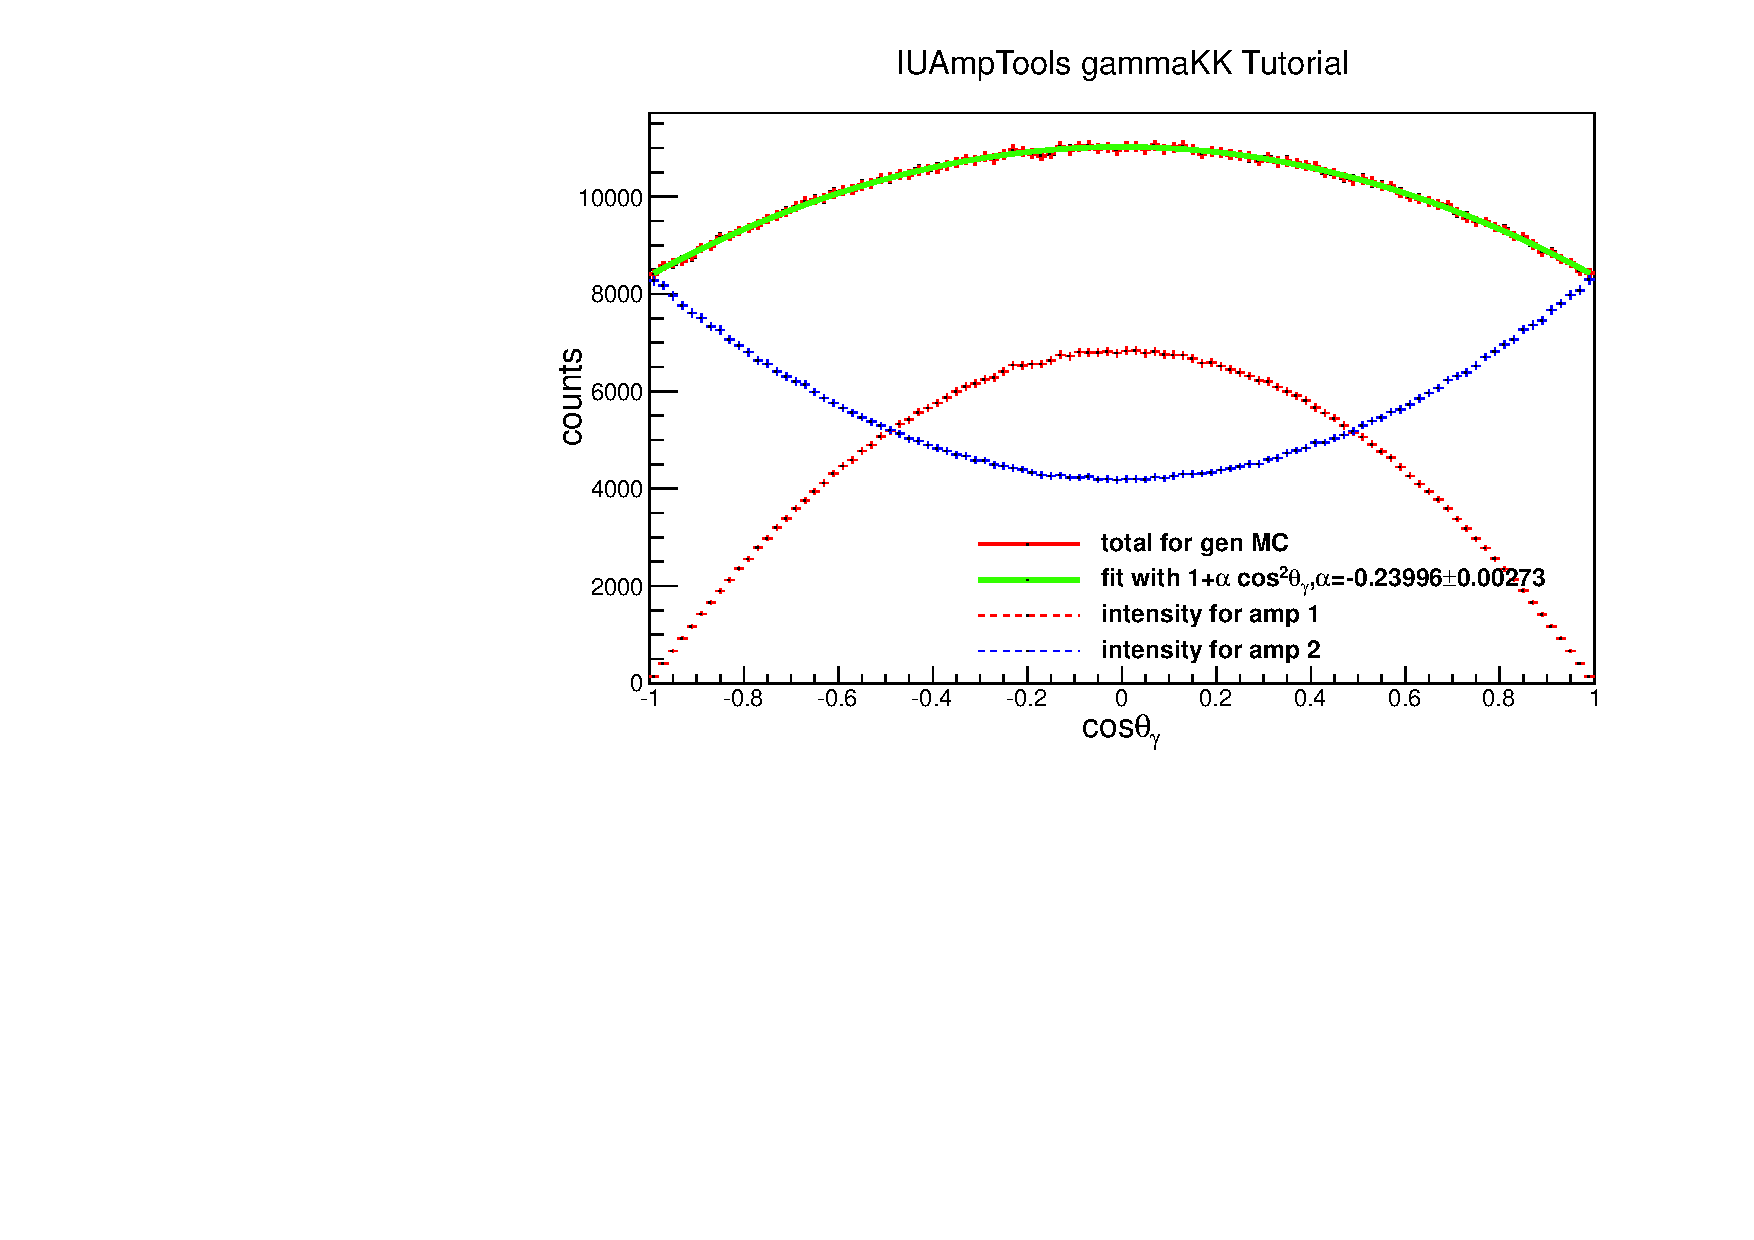
\includegraphics[width=0.9\columnwidth]{helicity_with_helicity.pdf}
    \end{minipage}
  }
  \hfill
  \subfloat{
    \begin{minipage}[c]{\textwidth}
      \centering
      \label{fig:helicity_with_multipole}
      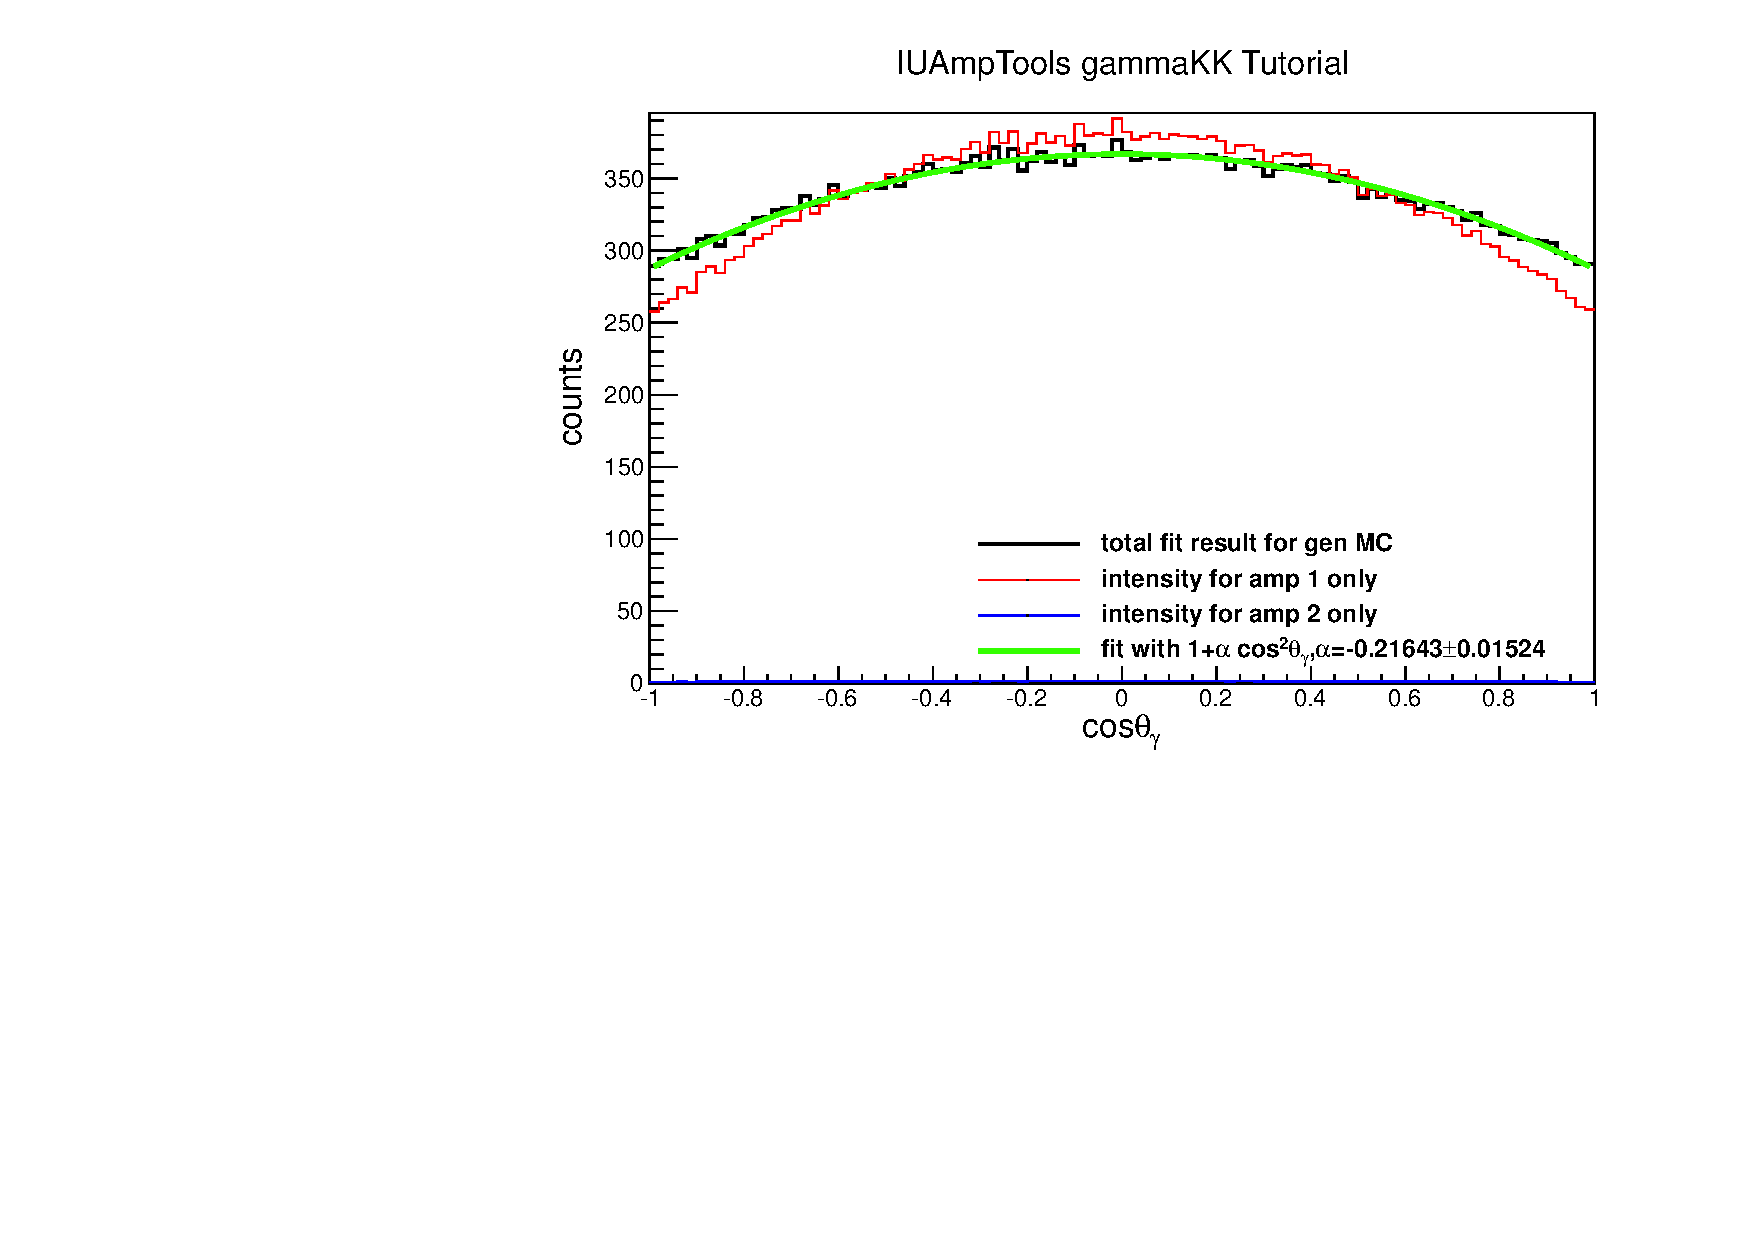
\includegraphics[width=0.9\columnwidth]{helicity_with_multipole.pdf}
    \end{minipage}
  }
  \caption{
    The angular distributions obtained for a mixture of helicity
    amplitudes, fit with helicity amplitudes (top) and multipole
    amplitudes (bottom). In both cases the correct parameter $\alpha$ for
    the distribution $1 + \alpha \cos^{2} \theta_{\gamma}$ is extracted
    from a fit, although the ampitudes contribute in significantly
    different ways. Note the dashed blue curve at the bottom for M2 in
    the bottom plot. The difference between the intensity of amp 1 (E1)
    and the total distribution is the interference between E1 and M2. In
    the example above, the ratio is $A_{1}/A_{0}=0.95/1.05$ where
    $A_{\mu}$ is the strength of the helicity amplitude for $\mu$.
  }
  \label{fig:fits_helicity}
\end{figure}

\begin{figure}
  \subfloat{
    \begin{minipage}[c]{\textwidth}
      \centering
      \label{fig:multipole_with_helicity}
      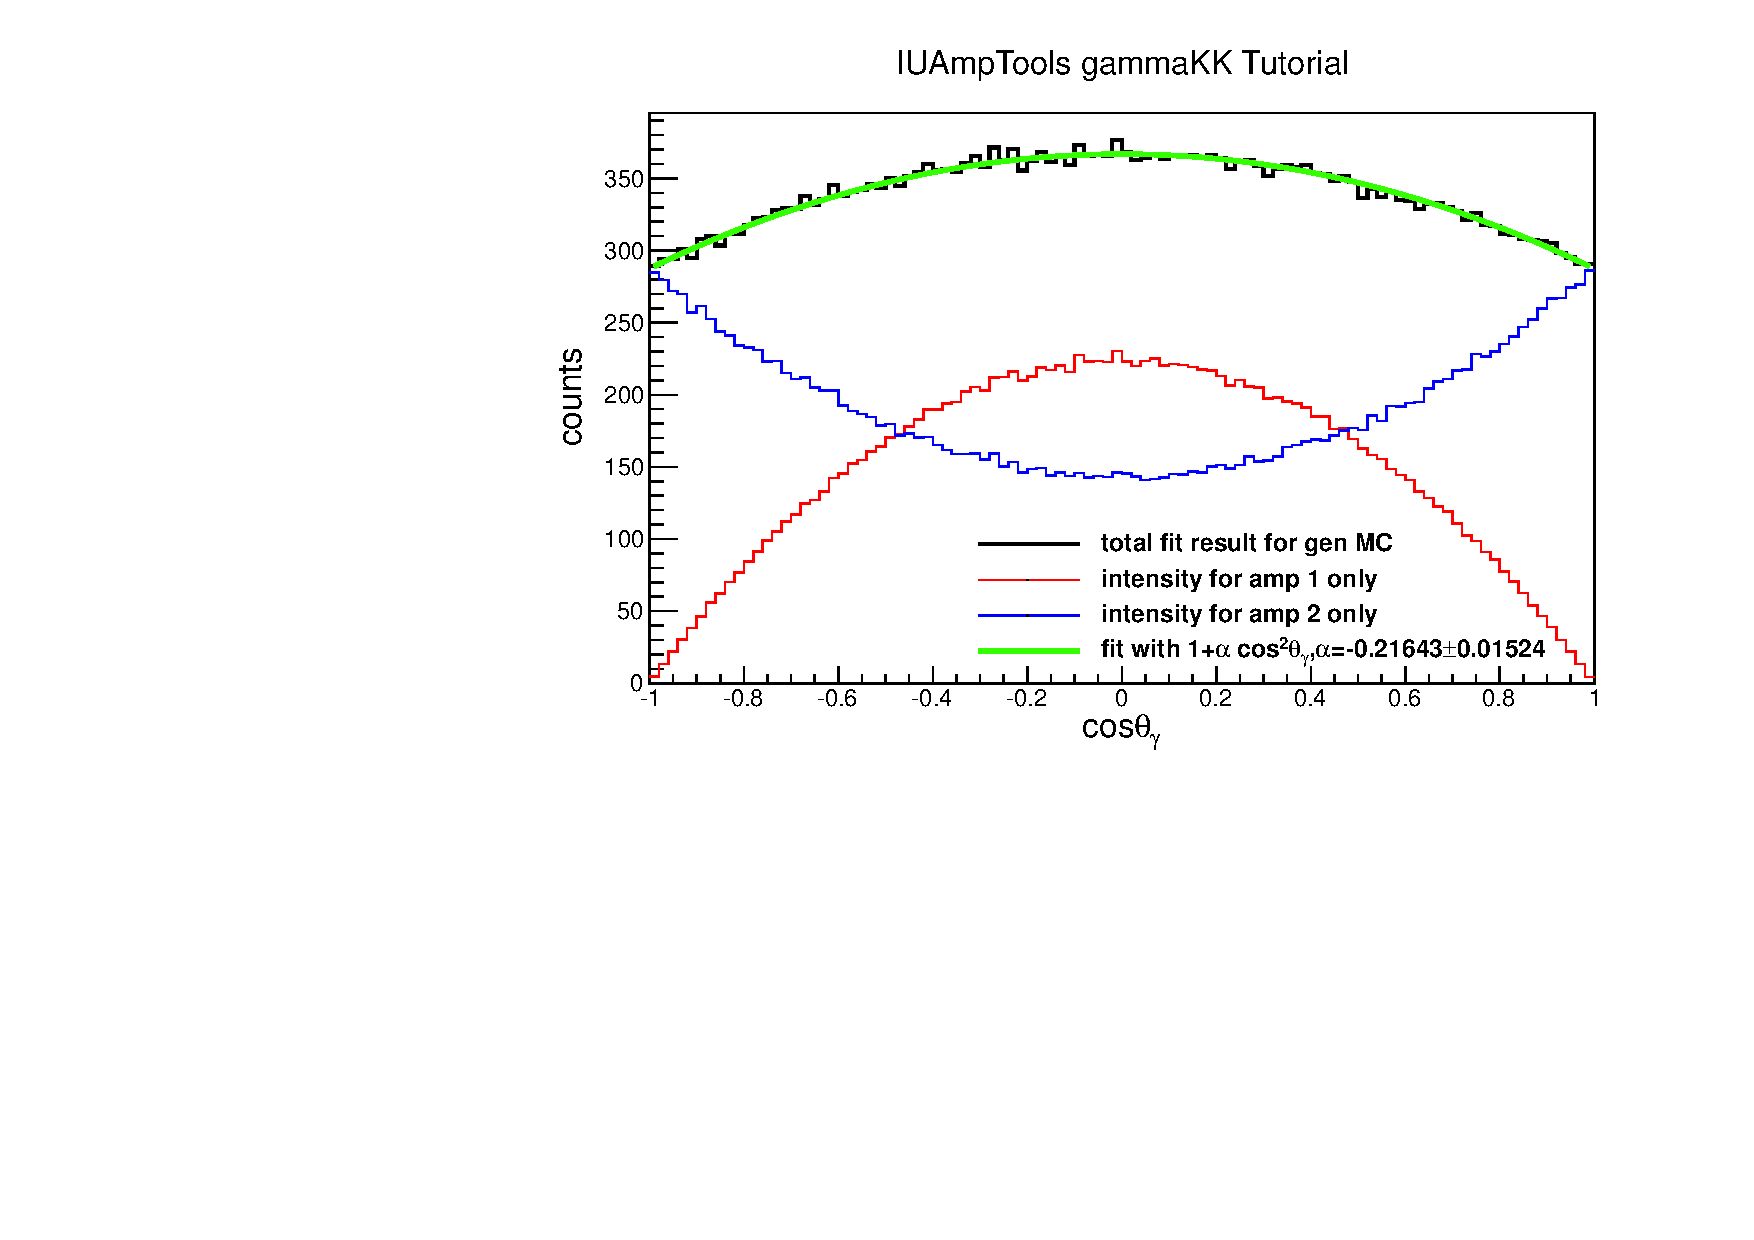
\includegraphics[width=0.9\columnwidth]{multipole_with_helicity.pdf}
    \end{minipage}
  }
  \hfill
  \subfloat{
    \begin{minipage}[c]{\textwidth}
      \centering
      \label{fig:multipole_with_multipole}
      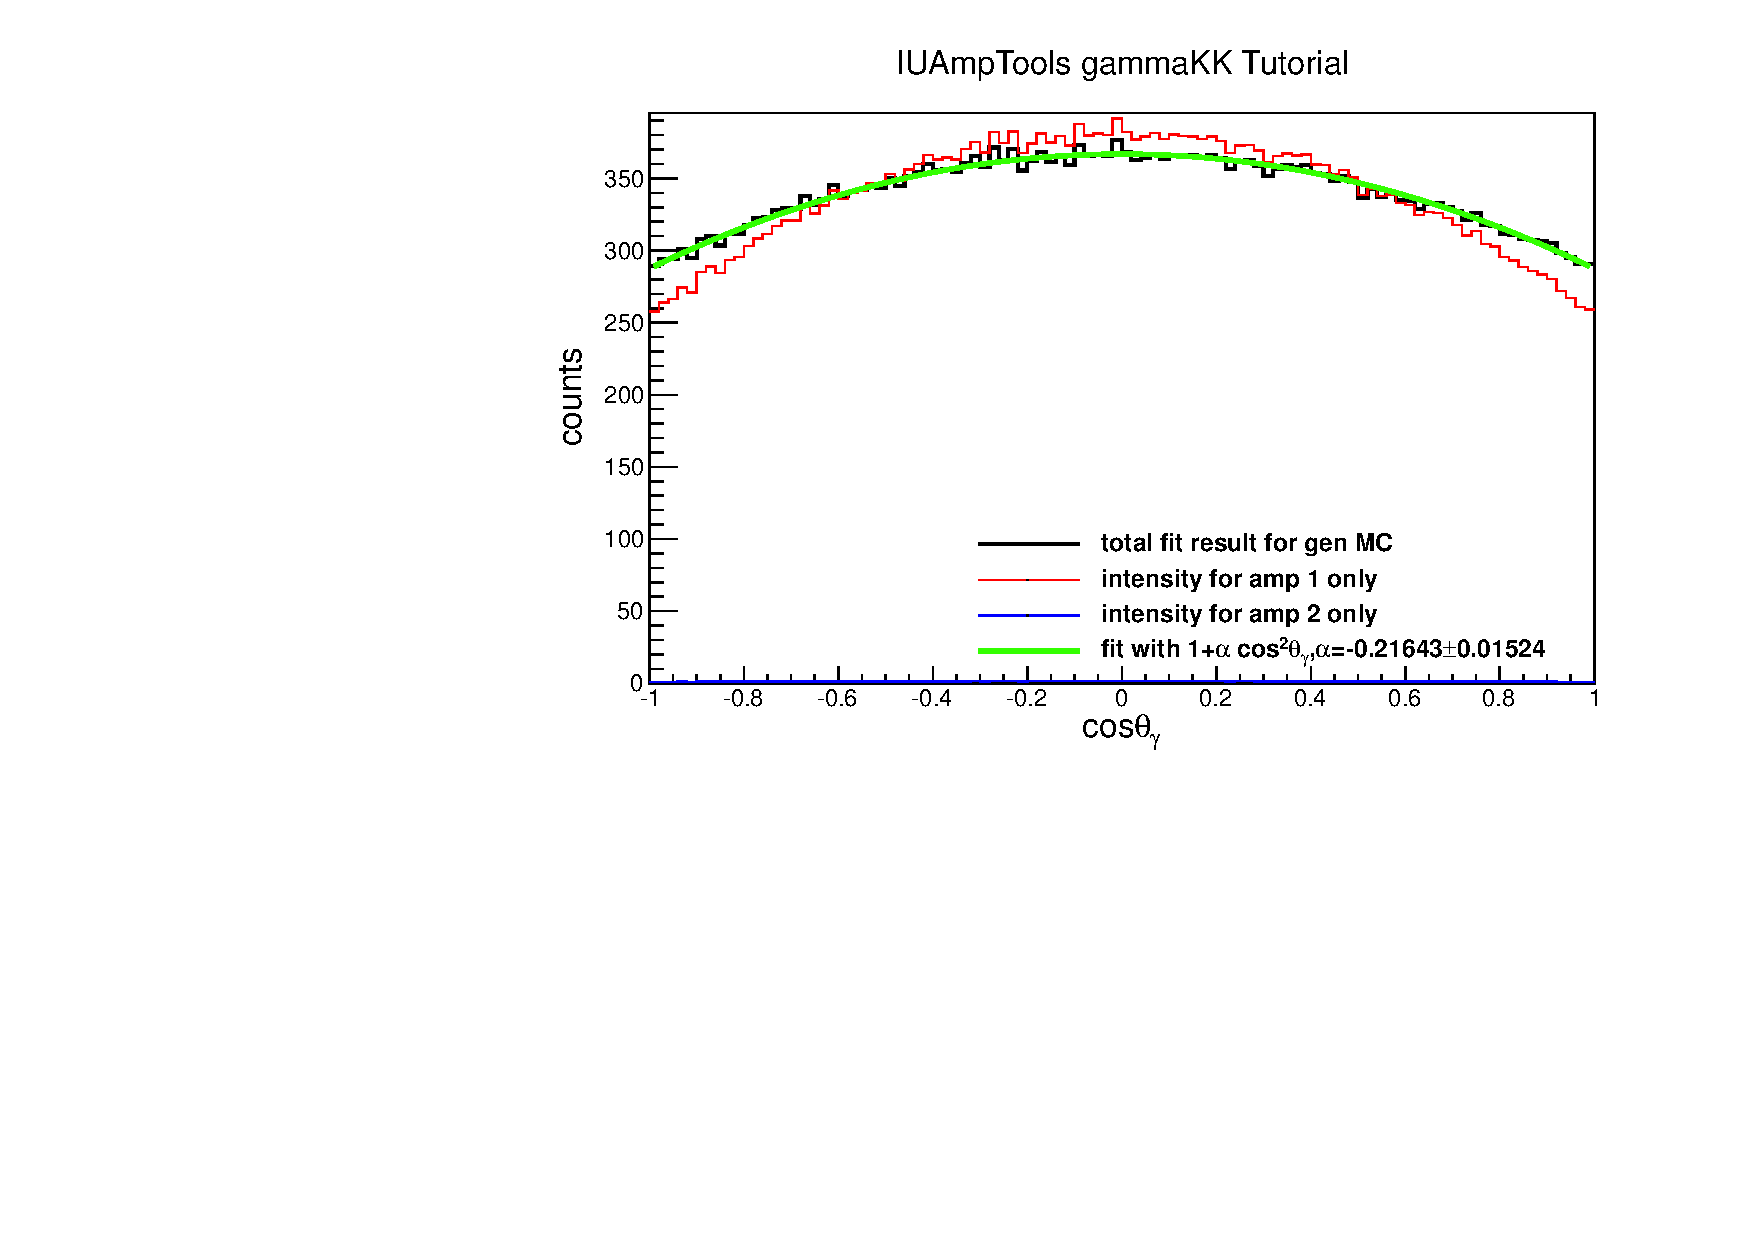
\includegraphics[width=0.9\columnwidth]{multipole_with_multipole.pdf}
    \end{minipage}
  }
  \caption{
    The angular distributions obtained for a mixture of E1 and M2
    amplitudes, fit with helicity amplitudes (top) and multipole
    amplitudes (bottom). In both cases the correct parameter $\alpha$ for
    the distribution $1 + \alpha \cos^{2} \theta_{\gamma}$ is extracted
    from a fit, although the ampitudes contribute in significantly
    different ways. Note the dashed blue curve at the bottom for M2 in
    the bottom plot. The difference between the intensity of amp 1 (E1)
    and the total distribution is the interference between E1 and M2. In
    the example above, the ratio is M2/E1$=0.05$.
  }
  \label{fig:fits_multipole}
\end{figure}

%*************************************************************************************
%                                                                                    *
%                                    Conclusions                                     *
%                                                                                    *
%*************************************************************************************
\section{Conclusion}

This document summarizes the usage of the tutorial to do a
mass-independent amplitude analysis of $J/\psi \to \gamma KK$ using
\AmpTools. The scripts included should allow the user to understand
what is going on inside each step of the program.

% Create the reference section using BibTeX:
% \bibliography{lineshape}

%*************************************************************************************
%                                                                                    *
%                                     Appendix                                       *
%                                                                                    *
%*************************************************************************************
%% \appendix
%% 
%% \section{Appendix}
%% 
%% This Appendix is a reference for multipole transition papers in
%% charmonium for people interested in the multipole expansion.
%% 
%% \subsection{Experimental Papers}
%% There have been many papers that discuss the multipole amplitudes of
%% charmonium, some of which are listed below.
%% 
%% \begin{enumerate}
%% 
%% \item Crystal Ball@SLAC (1982)
%% \item CLEO-c (2009)
%% \item BESIII (2011)
%% \end{enumerate}
%% 
%% 
%% \subsection{Theory Papers}
 
\end{document}
